%% bare_conf.tex
%% V1.4b
%% 2015/08/26
%% by Michael Shell
%% See:
%% http://www.michaelshell.org/
%% for current contact information.
%%
%% This is a skeleton file demonstrating the use of IEEEtran.cls
%% (requires IEEEtran.cls version 1.8b or later) with an IEEE
%% conference paper.
%%
%% Support sites:
%% http://www.michaelshell.org/tex/ieeetran/
%% http://www.ctan.org/pkg/ieeetran
%% and
%% http://www.ieee.org/

%%*************************************************************************
%% Legal Notice:
%% This code is offered as-is without any warranty either expressed or
%% implied; without even the implied warranty of MERCHANTABILITY or
%% FITNESS FOR A PARTICULAR PURPOSE! 
%% User assumes all risk.
%% In no event shall the IEEE or any contributor to this code be liable for
%% any damages or losses, including, but not limited to, incidental,
%% consequential, or any other damages, resulting from the use or misuse
%% of any information contained here.
%%
%% All comments are the opinions of their respective authors and are not
%% necessarily endorsed by the IEEE.
%%
%% This work is distributed under the LaTeX Project Public License (LPPL)
%% ( http://www.latex-project.org/ ) version 1.3, and may be freely used,
%% distributed and modified. A copy of the LPPL, version 1.3, is included
%% in the base LaTeX documentation of all distributions of LaTeX released
%% 2003/12/01 or later.
%% Retain all contribution notices and credits.
%% ** Modified files should be clearly indicated as such, including  **
%% ** renaming them and changing author support contact information. **
%%*************************************************************************


% *** Authors should verify (and, if needed, correct) their LaTeX system  ***
% *** with the testflow diagnostic prior to trusting their LaTeX platform ***
% *** with production work. The IEEE's font choices and paper sizes can   ***
% *** trigger bugs that do not appear when using other class files.       ***                          ***
% The testflow support page is at:
% http://www.michaelshell.org/tex/testflow/



\documentclass[conference]{IEEEtran}
% Some Computer Society conferences also require the compsoc mode option,
% but others use the standard conference format.
%
% If IEEEtran.cls has not been installed into the LaTeX system files,
% manually specify the path to it like:
% \documentclass[conference]{../sty/IEEEtran}





% Some very useful LaTeX packages include:
% (uncomment the ones you want to load)


% *** MISC UTILITY PACKAGES ***
%
%\usepackage{ifpdf}
% Heiko Oberdiek's ifpdf.sty is very useful if you need conditional
% compilation based on whether the output is pdf or dvi.
% usage:
% \ifpdf
%   % pdf code
% \else
%   % dvi code
% \fi
% The latest version of ifpdf.sty can be obtained from:
% http://www.ctan.org/pkg/ifpdf
% Also, note that IEEEtran.cls V1.7 and later provides a builtin
% \ifCLASSINFOpdf conditional that works the same way.
% When switching from latex to pdflatex and vice-versa, the compiler may
% have to be run twice to clear warning/error messages.






% *** CITATION PACKAGES ***
%
\usepackage{cite}
% cite.sty was written by Donald Arseneau
% V1.6 and later of IEEEtran pre-defines the format of the cite.sty package
% \cite{} output to follow that of the IEEE. Loading the cite package will
% result in citation numbers being automatically sorted and properly
% "compressed/ranged". e.g., [1], [9], [2], [7], [5], [6] without using
% cite.sty will become [1], [2], [5]--[7], [9] using cite.sty. cite.sty's
% \cite will automatically add leading space, if needed. Use cite.sty's
% noadjust option (cite.sty V3.8 and later) if you want to turn this off
% such as if a citation ever needs to be enclosed in parenthesis.
% cite.sty is already installed on most LaTeX systems. Be sure and use
% version 5.0 (2009-03-20) and later if using hyperref.sty.
% The latest version can be obtained at:
% http://www.ctan.org/pkg/cite
% The documentation is contained in the cite.sty file itself.






% *** GRAPHICS RELATED PACKAGES ***
%
\ifCLASSINFOpdf
  \usepackage[pdftex]{graphicx}
  % declare the path(s) where your graphic files are
  % \graphicspath{{../pdf/}{../jpeg/}}
  % and their extensions so you won't have to specify these with
  % every instance of \includegraphics
  % \DeclareGraphicsExtensions{.pdf,.jpeg,.png}
\else
  % or other class option (dvipsone, dvipdf, if not using dvips). graphicx
  % will default to the driver specified in the system graphics.cfg if no
  % driver is specified.
  % \usepackage[dvips]{graphicx}
  % declare the path(s) where your graphic files are
  % \graphicspath{{../eps/}}
  % and their extensions so you won't have to specify these with
  % every instance of \includegraphics
  % \DeclareGraphicsExtensions{.eps}
\fi
% graphicx was written by David Carlisle and Sebastian Rahtz. It is
% required if you want graphics, photos, etc. graphicx.sty is already
% installed on most LaTeX systems. The latest version and documentation
% can be obtained at: 
% http://www.ctan.org/pkg/graphicx
% Another good source of documentation is "Using Imported Graphics in
% LaTeX2e" by Keith Reckdahl which can be found at:
% http://www.ctan.org/pkg/epslatex
%
% latex, and pdflatex in dvi mode, support graphics in encapsulated
% postscript (.eps) format. pdflatex in pdf mode supports graphics
% in .pdf, .jpeg, .png and .mps (metapost) formats. Users should ensure
% that all non-photo figures use a vector format (.eps, .pdf, .mps) and
% not a bitmapped formats (.jpeg, .png). The IEEE frowns on bitmapped formats
% which can result in "jaggedy"/blurry rendering of lines and letters as
% well as large increases in file sizes.
%
% You can find documentation about the pdfTeX application at:
% http://www.tug.org/applications/pdftex





% *** MATH PACKAGES ***
%
\usepackage{amsmath}
% A popular package from the American Mathematical Society that provides
% many useful and powerful commands for dealing with mathematics.
%
% Note that the amsmath package sets \interdisplaylinepenalty to 10000
% thus preventing page breaks from occurring within multiline equations. Use:
%\interdisplaylinepenalty=2500
% after loading amsmath to restore such page breaks as IEEEtran.cls normally
% does. amsmath.sty is already installed on most LaTeX systems. The latest
% version and documentation can be obtained at:
% http://www.ctan.org/pkg/amsmath





% *** SPECIALIZED LIST PACKAGES ***
%
%\usepackage{algorithmic}
% algorithmic.sty was written by Peter Williams and Rogerio Brito.
% This package provides an algorithmic environment fo describing algorithms.
% You can use the algorithmic environment in-text or within a figure
% environment to provide for a floating algorithm. Do NOT use the algorithm
% floating environment provided by algorithm.sty (by the same authors) or
% algorithm2e.sty (by Christophe Fiorio) as the IEEE does not use dedicated
% algorithm float types and packages that provide these will not provide
% correct IEEE style captions. The latest version and documentation of
% algorithmic.sty can be obtained at:
% http://www.ctan.org/pkg/algorithms
% Also of interest may be the (relatively newer and more customizable)
% algorithmicx.sty package by Szasz Janos:
% http://www.ctan.org/pkg/algorithmicx




% *** ALIGNMENT PACKAGES ***
%
%\usepackage{array}
% Frank Mittelbach's and David Carlisle's array.sty patches and improves
% the standard LaTeX2e array and tabular environments to provide better
% appearance and additional user controls. As the default LaTeX2e table
% generation code is lacking to the point of almost being broken with
% respect to the quality of the end results, all users are strongly
% advised to use an enhanced (at the very least that provided by array.sty)
% set of table tools. array.sty is already installed on most systems. The
% latest version and documentation can be obtained at:
% http://www.ctan.org/pkg/array


% IEEEtran contains the IEEEeqnarray family of commands that can be used to
% generate multiline equations as well as matrices, tables, etc., of high
% quality.




% *** SUBFIGURE PACKAGES ***
%\ifCLASSOPTIONcompsoc
%  \usepackage[caption=false,font=normalsize,labelfont=sf,textfont=sf]{subfig}
%\else
%  \usepackage[caption=false,font=footnotesize]{subfig}
%\fi
% subfig.sty, written by Steven Douglas Cochran, is the modern replacement
% for subfigure.sty, the latter of which is no longer maintained and is
% incompatible with some LaTeX packages including fixltx2e. However,
% subfig.sty requires and automatically loads Axel Sommerfeldt's caption.sty
% which will override IEEEtran.cls' handling of captions and this will result
% in non-IEEE style figure/table captions. To prevent this problem, be sure
% and invoke subfig.sty's "caption=false" package option (available since
% subfig.sty version 1.3, 2005/06/28) as this is will preserve IEEEtran.cls
% handling of captions.
% Note that the Computer Society format requires a larger sans serif font
% than the serif footnote size font used in traditional IEEE formatting
% and thus the need to invoke different subfig.sty package options depending
% on whether compsoc mode has been enabled.
%
% The latest version and documentation of subfig.sty can be obtained at:
% http://www.ctan.org/pkg/subfig




% *** FLOAT PACKAGES ***
%
%\usepackage{fixltx2e}
% fixltx2e, the successor to the earlier fix2col.sty, was written by
% Frank Mittelbach and David Carlisle. This package corrects a few problems
% in the LaTeX2e kernel, the most notable of which is that in current
% LaTeX2e releases, the ordering of single and double column floats is not
% guaranteed to be preserved. Thus, an unpatched LaTeX2e can allow a
% single column figure to be placed prior to an earlier double column
% figure.
% Be aware that LaTeX2e kernels dated 2015 and later have fixltx2e.sty's
% corrections already built into the system in which case a warning will
% be issued if an attempt is made to load fixltx2e.sty as it is no longer
% needed.
% The latest version and documentation can be found at:
% http://www.ctan.org/pkg/fixltx2e


%\usepackage{stfloats}
% stfloats.sty was written by Sigitas Tolusis. This package gives LaTeX2e
% the ability to do double column floats at the bottom of the page as well
% as the top. (e.g., "\begin{figure*}[!b]" is not normally possible in
% LaTeX2e). It also provides a command:
%\fnbelowfloat
% to enable the placement of footnotes below bottom floats (the standard
% LaTeX2e kernel puts them above bottom floats). This is an invasive package
% which rewrites many portions of the LaTeX2e float routines. It may not work
% with other packages that modify the LaTeX2e float routines. The latest
% version and documentation can be obtained at:
% http://www.ctan.org/pkg/stfloats
% Do not use the stfloats baselinefloat ability as the IEEE does not allow
% \baselineskip to stretch. Authors submitting work to the IEEE should note
% that the IEEE rarely uses double column equations and that authors should try
% to avoid such use. Do not be tempted to use the cuted.sty or midfloat.sty
% packages (also by Sigitas Tolusis) as the IEEE does not format its papers in
% such ways.
% Do not attempt to use stfloats with fixltx2e as they are incompatible.
% Instead, use Morten Hogholm'a dblfloatfix which combines the features
% of both fixltx2e and stfloats:
%
% \usepackage{dblfloatfix}
% The latest version can be found at:
% http://www.ctan.org/pkg/dblfloatfix




% *** PDF, URL AND HYPERLINK PACKAGES ***
%
\usepackage{url}
% url.sty was written by Donald Arseneau. It provides better support for
% handling and breaking URLs. url.sty is already installed on most LaTeX
% systems. The latest version and documentation can be obtained at:
% http://www.ctan.org/pkg/url
% Basically, \url{my_url_here}.




% *** Do not adjust lengths that control margins, column widths, etc. ***
% *** Do not use packages that alter fonts (such as pslatex).         ***
% There should be no need to do such things with IEEEtran.cls V1.6 and later.
% (Unless specifically asked to do so by the journal or conference you plan
% to submit to, of course. )


% correct bad hyphenation here
\hyphenation{op-tical net-works semi-conduc-tor}


\begin{document}
%
% paper title
% Titles are generally capitalized except for words such as a, an, and, as,
% at, but, by, for, in, nor, of, on, or, the, to and up, which are usually
% not capitalized unless they are the first or last word of the title.
% Linebreaks \\ can be used within to get better formatting as desired.
% Do not put math or special symbols in the title.
\title{Deep Learning for Time-Series Analysis\\ of Sleep State Detection \\ in Wrist-Worn Devices}


% author names and affiliations
% use a multiple column layout for up to three different
% affiliations
\author{\IEEEauthorblockN{Armando Bringas-Corpus}
\IEEEauthorblockA{Escuela de Ingeniería y Ciencias\\
Tecnológico de Monterrey\\
Querétaro, México\\
Email: a01200230@tec.mx}}

% conference papers do not typically use \thanks and this command
% is locked out in conference mode. If really needed, such as for
% the acknowledgment of grants, issue a \IEEEoverridecommandlockouts
% after \documentclass

% for over three affiliations, or if they all won't fit within the width
% of the page, use this alternative format:
% 
%\author{\IEEEauthorblockN{Michael Shell\IEEEauthorrefmark{1},
%Homer Simpson\IEEEauthorrefmark{2},
%James Kirk\IEEEauthorrefmark{3}, 
%Montgomery Scott\IEEEauthorrefmark{3} and
%Eldon Tyrell\IEEEauthorrefmark{4}}
%\IEEEauthorblockA{\IEEEauthorrefmark{1}School of Electrical and Computer Engineering\\
%Georgia Institute of Technology,
%Atlanta, Georgia 30332--0250\\ Email: see http://www.michaelshell.org/contact.html}
%\IEEEauthorblockA{\IEEEauthorrefmark{2}Twentieth Century Fox, Springfield, USA\\
%Email: homer@thesimpsons.com}
%\IEEEauthorblockA{\IEEEauthorrefmark{3}Starfleet Academy, San Francisco, California 96678-2391\\
%Telephone: (800) 555--1212, Fax: (888) 555--1212}
%\IEEEauthorblockA{\IEEEauthorrefmark{4}Tyrell Inc., 123 Replicant Street, Los Angeles, California 90210--4321}}




% use for special paper notices
%\IEEEspecialpapernotice{(Invited Paper)}




% make the title area
\maketitle

% As a general rule, do not put math, special symbols or citations
% in the abstract
\begin{abstract}
This investigation proposes a project that utilizes deep learning techniques to address the complex task of detecting sleep states using accelerometer data from wrist-worn devices. This research include a review and critical evaluation of various deep learning architectures, comparing them with other machine learning strategies to determine the most effective approach. With an initial focus on examining state-of-the-art methods, central to this proposal is the development of a deep learning solution for analyzing and predicting time-series data from these wrist-worn devices to accurately identify sleep states. The overarching aim is to implement a reliable predictive model that significantly enhances the precision and dependability of sleep state classification using data from wearable technology.
\end{abstract}

% no keywords




% For peer review papers, you can put extra information on the cover
% page as needed:
% \ifCLASSOPTIONpeerreview
% \begin{center} \bfseries EDICS Category: 3-BBND \end{center}
% \fi
%
% For peerreview papers, this IEEEtran command inserts a page break and
% creates the second title. It will be ignored for other modes.
\IEEEpeerreviewmaketitle



\section{Introduction}

This paper presents a project proposal rooted in the practical application of a Kaggle competition, aimed at addressing a challenge in pediatric health and neuroscience: the identification of sleep states in children through wrist-worn accelerometer data. The competition serves as a catalyst for innovation, prompting the development of a sophisticated machine learning model capable of discerning the subtle onset of various sleep states and periods of wakefulness with precision.

The significance of this project lies in its potential to deepen our understanding of sleep and to provide further insights into its importance. For instance, understanding how environmental factors influence sleep, mood, and behavior can aid in formulating personalized strategies tailored to the unique needs of each child \cite{child-mind-institute-detect-sleep-states}. Furthermore, the outcomes of this project could enable researchers to undertake more comprehensive, large-scale sleep studies across a variety of populations and contexts, which could yield even more valuable information about sleep \cite{child-mind-institute-detect-sleep-states}.
  

\section{Literature Review}

For this type of problem, a Machine Learning approach based on Random Forest has proven effective in detecting sleep-wake states, non-wear versus wear, and sleep stage classification \cite{Sundararajan2021}. An initial attempt was made using a Residual Neural Network (RNN), specifically a ResNet initialized with a Glorot uniform initializer and employing LeakyReLU activations \cite{Sundararajan2021}. However, when testing this approach with the Amsterdam dataset, which consists of data collected from 114 individuals recruited by the VU University Medical Center in Amsterdam, The Netherlands \cite{teLindert2020}, it was observed that the Random Forest approach outperformed the ResNet heuristic. Notably, the ResNet had difficulties with wake state prediction \cite{Sundararajan2021}. However, it is important to remark that most the used data was collected with the GENActiv accelerometer brand, it should be consider future studies to assess model transferability across other accelerometer brands \cite{Sundararajan2021}.

We explored another approach that analyzes data from the VU University Medical Center in Amsterdam, The Netherlands \cite{teLindert2020}. Unlike machine learning methods, this study employed Latent Class Analysis (LCA), a statistical method rather than a machine learning or deep learning technique. LCA, commonly used in social, psychological, and behavioral sciences, identifies latent classes within populations sharing common characteristics \cite{qing2023}. In their study, LCA was utilized to differentiate subtypes of sleep misperception among individuals using data from actigraphy and sleep diaries from the people in their studies \cite{teLindert2020}. Sleep misperception, in this context, is the discrepancy between subjectively perceived and objectively measured sleep, crucial for understanding disorders like Insomnia Disorder \cite{teLindert2020}. This study, focusing on a statistical categorical approach to classify sleep misperception, falls outside our scope.

Also, it is important to note that the analyzed information for sleep state detection can come from different types of devices, from example from an optical plethysmography and accelerometer signals \cite{Beattie_2017} \cite{Fedorin2019}, depending on the research. Specifically, there are cases in which the data is extracted from accelerometers among other types of sensors. Therefore, the methods utilized in each case serve as a baseline for their respective projects, this means that couldn't be possible a suitable that generalize over the data coming from different sources.

Understanding the clinical implications of devices employed for sleep state detection is crucial. Accelerometry is frequently utilized as a cost-effective method for assessing sleep states. However, it appears that traditional machine learning algorithms may have limitations in accuracy, particularly in patients with insomnia \cite{Sundararajan2021}. There exists both an opportunity and a growing interest in refining these algorithms by enhancing the accuracy of accelerometry could transform it into a more clinically valuable tool, enabling the measurement of sleep and wakefulness over prolonged periods \cite{Sundararajan2021}.

Despite evidence suggesting that classical methods, such as Support Vector Machines, effectively detect sleep states and may outperform Deep Learning methods in specific scenarios with data from actigraph devices that recorded signals using a microelectromechanical system (MEMS) accelerometer \cite{teLindert2020}, similar to the GENActiv accelerometer \cite{Sundararajan2021}, were analyzed., we explored alternative approaches. Our investigation revealed the deployment of Deep Learning and other Machine Learning models for detecting sleep states from various source signals. These include electrocardiography (ECG), which measures the heart's electrical activity in combination of respiratory and movement signals \cite{Stuburic2020}, or electroencephalogram (EEG), employing electrodes on the scalp to monitor brain electrical signals \cite{Sekkal2022}. Other sources involve a combination of optical plethysmography and accelerometer signals \cite{Beattie_2017} \cite{Fedorin2019}, and more complex inputs like multi-channel polysomnogram (PSG) \cite{Li2021}. PSG encompasses diverse physiological continuous-time signals from multiple sensors, including EEG, electrooculography (EOG) for eye movement, electromyography (EMG) for muscle contractions, and monitors for respiration and body oxygen levels \cite{Li2021}.

Although the different source signals, overally, they shared in common the complexity, high-dimensionality, noise and temporo-spatial dependency structure of these data types that make them suitable for analysis using deep learning models with their respective challenges \cite{thomas2018}. A potential challenge could yield with working with raw signals introduced with the network without doing feature extraction \cite{Stuburic2020}. From the work of \cite{michielli2019} they compare different methods and algorithms based on data from heart rate and wrist actigraphy, but they did low-level and mid-level feature extraction before introducing to the network, the best results was obtained from a Long Short-Term Memory LSTM network for 2-class classification with an accuracy of 83.56\% \cite{michielli2019}.

A Long Short-Term Memory network (LSTM) is a specialized type of Recurrent Neural Network (RNN). It's important to note that RNNs are a natural choice for time-series forecasting and prediction \cite{Aggarwal2018}. LSTM enhances the RNN architecture by modifying the recurrence conditions of how the hidden states are propagated \cite{Aggarwal2018}. Additionally, it addresses the challenges of vanishing and exploding gradients, which are critical issues in neural network training \cite{Aggarwal2018, michielli2019}.

In their research, Sekkal et al. \cite{Sekkal2022} utilized a LSTM network for analyzing the Physionet Sleep-EDF Database, containing 153 polysomnograms (PSGs) from two-night recordings. Feature extraction was performed to refine the data within the PSG signals. The study's relevance stems from its comparison of classical machine learning techniques with deep learning approaches, notably focusing on LSTM due to its proficiency in identifying temporal relationships between sleep stages \cite{Sekkal2022}. In their bi-directional LSTM classifier implementation, an accuracy of 87.8\% was achieved on the PSG (Fpz-Cz + Pz-Oz + EOG) classifier. Contrasting this, Fraiwan \& Alkhodari \cite{fraiwan2020} reported a peak accuracy of 97.1\% using a bi-directional LSTM with a single channel. However, their training set showed significant class imbalance, with the 'awake' stage constituting 68\% of the epochs. This imbalance likely skewed the classifier's performance, favoring the more prevalent sleep stage.

The bi-directional LSTM classifier model, referenced in the studies by Sekkal et al. \cite{Sekkal2022} and Fraiwan \& Alkhodari \cite{fraiwan2020}, represents an enhancement of the standard LSTM. This variant eliminates the one-step truncation inherent in the original LSTM design. Bidirectional training possesses an architectural advantage over unidirectional training if used
to classify phonemes \cite{Graves2005}, it incorporates a comprehensive error gradient calculation, enabling training through standard backpropagation through time (BPTT) \cite{Staudemeyer2019}.

Is important to remark that Fiorillo et al. \cite{Fiorillo2019} present a systematic and comprehensive review of deep learning algorithms applied to sleep scoring. The paper thoroughly examines the latest applications and compares them to other methodologies, it concluded that deep learning methods offer numerous advantages. Notably, these algorithms can be applied directly to raw data in comparison with other approaches that involved feature extraction \cite{Stuburic2020} \cite{michielli2019}, therefore requiring minimal artifact removal. Furthermore, they are capable of unveiling hidden information that traditional feature-based approaches might overlook.

Finally, in the work of \cite{Stuburic2020} they implemented a LSTM architecture with the raw signals from EEG without any prior feature extraction. The preprocessing involved reducing noise and smoothing the signal using a median filter and, in some cases, applying signal flipping or baseline subtraction. LSTM were designed to learn features directly from these raw, preprocessed signals without any feature extraction step, they achieved an accuracy of 80\% in 5-class classification.

To address our particular challenge, we propose initially implementing an LSTM architecture without feature extraction. This approach is selected based on revisited literature that emphasizes its effectiveness in capturing temporal dependencies in sequential data, a key characteristic of our problem domain. Subsequent stages of our research will involve evaluating the performance of this model and discussing potential enhancements. These may include the integration of feature extraction techniques or the exploration of other Deep Learning architectures, as needed.


\section{Future Directions}

The ultimate goal is to apply a developed Deep Learning architecture to the dataset provided by \cite{child-mind-institute-detect-sleep-states}. Our primary motivation lies in the use of deep learning methods for time series analysis, particularly with the "Detect Sleep States" dataset furnished by the Child Mind Institute \cite{child-mind-institute-detect-sleep-states}. 


\subsection{Data}

 \begin{figure*}[ht]
    \centering
    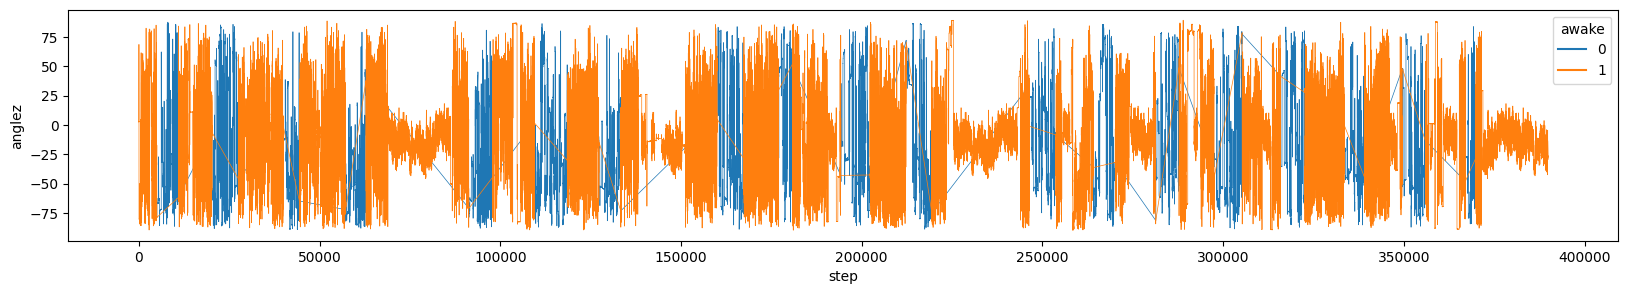
\includegraphics[width=1\linewidth]{TC5033_Activity_5-State_of_the_art_research/figures/time_series.png}
    \caption{Accelerometer training data. Plot of \texttt{step} againts \texttt{anglez} showing \texttt{event} state}
    \label{fig:accelerometerdata}
\end{figure*}

 The dataset consists of approximately 500 multi-day recordings from wrist-mounted accelerometers. The accelerometer data in the dataset was processed using R with the GGIR package \cite{Migueles2019GGIR}. The recordings are labeled with two event types: 'onset', indicating the start of sleep, and 'wakeup', marking its end. The primary objective is to identify these two events within the accelerometer data series, this primarily represents a binary classification task. As shown in Figue \ref{fig:accelerometerdata} The data represents series of continuous recording of the accelerometer data for a single subject spanning many days, where we can find:



 \begin{itemize}
  \item \texttt{series\_id}: Unique identifier for each accelerometer series.
    \item \texttt{step}: An integer timestep for each observation within a series. It is uniqute within a series
  \item \texttt{event}: The type of event, whether onset or wakeup. 
  \item \texttt{anglez}: As calculated and described by the GGIR package, z-angle is a metric derived from individual accelerometer components that is commonly used in sleep detection, and refers to the angle of the arm relative to the vertical axis of the body \cite{Migueles2019GGIR}.
  \item \texttt{enmo}: As calculated and described by the GGIR package, ENMO is the Euclidean Norm Minus One of all accelerometer signals, with negative values rounded to zero. While no standard measure of acceleration exists in this space, this is one of the several commonly computed features \cite{Migueles2019GGIR}.
\end{itemize}



\subsection{Model}

We are planning to implement an architecture that incorporates an LSTM cell into our sequence of input data. In this cell architecture, the intermediate variables \( \overline{i}, \overline{f}, \overline{o} \), corresponding to the \textit{input}, \textit{forget}, and \textit{output} gates, play crucial roles in updating the cell and hidden states. The determination of the hidden state vector \( \overline{h}^{(k)}_{t} \) and the cell state vector \( \overline{c}^{(k)}_{t} \) is a multi-step process that starts by computing the intermediate variables, followed by the computation of the hidden states from these intermediates \cite{Aggarwal2018}. The updates are as follows:

\vspace{0.5em}

\textbf{[Setting up intermediates]}
\begin{align*}
\begin{matrix}
\text{Input Gate:} \\
\text{Forget Gate:} \\
\text{Output Gate:} \\
\text{New C.-State:} \\
\end{matrix} &\begin{bmatrix}
\overline{i} \\ 
\overline{f} \\
\overline{o} \\
\overline{c} \\
\end{bmatrix} =
\begin{bmatrix}
\text{sigm} \\
\text{sigm} \\
\text{sigm} \\
\tanh \\
\end{bmatrix} W^{(k)}
\begin{bmatrix}
h_{t}^{(k-1)} \\
h_{t-1}^{(k)}
\end{bmatrix}
\end{align*}

\textbf{[Selectively forget and add to long-term memory]}

\begin{equation*}
\begin{aligned}
    \overline{c}^{(k)}_{t} = \overline{f} \odot \overline{c}^{(k)}_{t-1} + \overline{i} \odot \overline{c} \\
\end{aligned}
\end{equation*}

\textbf{[Selectively leak long-term memory to hidden state]}

\begin{equation*}
\begin{aligned}
    \overline{h}^{(k)}_{t} &= o_t \odot \tanh(\overline{c}^{(k)}_{t})
\end{aligned}
\end{equation*}

Our neural network architecture employs an LSTM to incorporate the classifications of previous inputs into the current sample's classification. This approach is suitable to looking back to inform the present, a method particularly suited for cyclical patterns like sleep stages \cite{Stuburic2020}, which recur throughout the night. Therefore, LSTMs, with their recurrent nature, could be an ideal choice for this type of cyclic temporal problems.

As shown in Figure \ref{fig:neuralnetwork} 
We are proposing a starting neural network architecture with the following blocks where consists of a LSTM layer of 64 units, ideal for processing sequences by capturing dependencies from prior inputs. This is followed by a Dense layer, the size of which matches the number of classification categories in your problem, in this case for our binary classification problem \(n_classes = 2\). The final component is a softmax activation function, applied to convert the output into a probability distribution across the predicted classes. 

\begin{figure}[h]
  \centering
  \[
  \xrightarrow{\text{input}} \boxed{\text{LSTM} (64)} \rightarrow \boxed{\text{Dense} (n_{\text{classes}})} \xrightarrow{\text{softmax}}
  \]
  \caption{Neural Network for accelerometer data classification}
  \label{fig:neuralnetwork}
\end{figure}


Is important to check if the impact to work directly with raw signals, the effects of the noise and the implications of not doing feature extraction do not affect performance in the training of the model. Subsequently, with the results of the first trials we might plan work more in data pre-processing if needed or even transition to more complex architectures. Other point of consideration is that one of the common problems is that the time-series sequences can be extremely long and therefore can be certain limitations with its performance \cite{Aggarwal2018}.


\subsection{Evaluation}

To evaluate model classification, predictions that align with the ground truth and exceed the threshold are labeled as True Positives (TP). Predictions that do not match are labeled as False Positives (FP), while ground truths without a corresponding prediction are labeled as False Negatives (FN). Where,

\[
\text{Score}(x) = 
\begin{cases} 
\text{TP} & \text{if }x \text{ matched and } x > \text{thresh.} \\
\text{FP} & \text{if }x \text{ unmatched pred.} \\
\text{FN} & \text{if }x \text{ unmatched truth} \\
\text{TN} & \text{otherwise}
\end{cases}
\]

It is necessary to compute the average precision \cite{child-mind-institute-detect-sleep-states}. By collecting the events within each \texttt{series\_id} from the data the Average Precision score will be computed for each \( \text{event} \times \text{tolerance} \) group \cite{child-mind-institute-detect-sleep-states}. The Average Precision is a measure that combines recall and precision for ranked retrieval results, for one information need, the average precision is the mean of the precision scores after each relevant document is retrieved \cite{Zhang2009}. Average Precision is defined as:

\begin{equation*}
    \text{AP} = \sum_n (R_n - R_{n-1}) P_n,
\end{equation*}

where \(P_n\) and \(R_n\) are the precision and recall at the nth threshold. With random predictions, the AP is the fraction of positive samples, the value from this function ranges from 0 and 1 and higher is better computed from the prediction scores, \cite{scikit-learn}\cite{flach2015}. Precision and Recall are computed as follows:

\begin{equation*}
    \text{precision} = \frac{tp}{tp + fp}, \quad
    \text{recall} = \frac{tp}{tp + fn} 
\end{equation*}

\vspace{.5em}

\section{Conclusion}

To address this challenge, we want to continue over implementing deep learning techniques, despite evidence from \cite{Sundararajan2021} indicating that traditional methods such as Random Forest outperform ResNets. Our motivation stems from the insights gained from \cite{Zhang2023}, where the authors present the Time-Series Neural Network (TNN). This method, which incorporates a Kernel Filter alongside a Time Attention Mechanism \cite{Zhang2023}, has demonstrated high accuracy in forecasting, will be interesting to evaluate their perfomance on classification. In our specific context, we are in the process of evaluating whether Long Short-Term Memory Networks (LSTM), Graph Neural Networks (GNN), or potentially an attention-based mechanism would be most suitable for our application.


% use section* for acknowledgment
\section*{Acknowledgment}


This project is being proposed during the Machine Learning Fall 2023 course with the Tsinghua University as part of the hybrid classroom experience in collaboration with Alexis Guerrero (alexis.guerrero@ug.uchile.cl) from the Universidad de Chile.





% trigger a \newpage just before the given reference
% number - used to balance the columns on the last page
% adjust value as needed - may need to be readjusted if
% the document is modified later
%\IEEEtriggeratref{8}
% The "triggered" command can be changed if desired:
%\IEEEtriggercmd{\enlargethispage{-5in}}

% references section

% can use a bibliography generated by BibTeX as a .bbl file
% BibTeX documentation can be easily obtained at:
% http://mirror.ctan.org/biblio/bibtex/contrib/doc/
% The IEEEtran BibTeX style support page is at:
% http://www.michaelshell.org/tex/ieeetran/bibtex/

% argument is your BibTeX string definitions and bibliography database(s)
\bibliography{TC5033_Activity_5-State_of_the_art_research/references}
\bibliographystyle{IEEEtran}

% <OR> manually copy in the resultant .bbl file
% set second argument of \begin to the number of references
% (used to reserve space for the reference number labels box)
%\begin{thebibliography}{1}

%\bibitem{IEEEhowto:kopka}
%H.~Kopka and P.~W. Daly, \emph{A Guide to \LaTeX}, 3rd~ed.\hskip 1em %plus
%  0.5em minus 0.4em\relax Harlow, England: Addison-Wesley, 1999.

%\end{thebibliography}




% that's all folks
\end{document}


